\documentclass[]{article}
\usepackage{caption,subcaption,graphicx,float,url,amsmath,amssymb,tocloft}
\usepackage[hidelinks]{hyperref}
\usepackage[toc,acronym,nonumberlist]{glossaries}
\setacronymstyle{long-short}
\usepackage{glossaries-extra}
\graphicspath{{figs/}} 
\setlength{\cftsubsecindent}{0em}
\setlength{\cftsecnumwidth}{3em}
\setlength{\cftsubsecnumwidth}{3em}

%opening
\title{
	Notes from Origins of Life\\
	Week 5: Evolution}
\author{Simon Crase}

\makeglossaries

\loadglsentries{glossary-entries}

\renewcommand{\thesection}{5.\arabic{section}}
\renewcommand{\glstextformat}[1]{\textbf{\em #1}}

\begin{document}

\maketitle

\begin{abstract}
   These are my notes from the $5^{th}$ Week of the Santa Fe Institute Origins of Life Course\cite{sfi2019}. The course aims to push the field of Origins of Life research forward by bringing new and synthetic thinking to the question of how life emerged from an abiotic world.\\
   The content and images contained herein are the intellectual property of the Santa Fe Institute, with the exception of any errors in transcription, which are my own.
   These notes are distributed in the hope that they will be useful,
   but without any warranty, and without even the implied warranty of
   merchantability or fitness for a particular purpose. All feedback is welcome,
   but I don't necessarily undertake to do anything with it.
\end{abstract}

\setcounter{tocdepth}{2}
\tableofcontents
\listoffigures

\section{Introduction}

We discuss Selection, Phylogenetics, Macroscopic Regularities across all of life, how has life evolved in creating Complexity, and evolutionary processes in Artificial Life. 

\section{Origins of Eukaryotes}

Lecturer: David Baum

Cellular life began prokaryotic: metabolic and genetic systems enclosed in a single
boundary

Eukaryotic cells evolved once

\begin{itemize}
	\item Many internal membrane-bound structures
	\begin{itemize}
		\item nucleus
		\item mitochondria
		\item endomembrane system)
	\end{itemize}
	\item A significant evolutionary event!
\end{itemize}

\begin{itemize}
	\item Cellular predators--Figure \ref{figs:Cellular:predators:symbiotic:hosts1}--the lions and tigers of the micro-biotic world!
	\item Symbiotic hosts--Figure \ref{figs:Cellular:predators:symbiotic:hosts2}-- the farmers of the micro-biotic world!
	\item Multicellularity
	\begin{itemize}
		\item why have only eukaryotes evolved multicellularity?
		\item Why have eukaryotes evolved it multiple times? The best known instances are animals, plants, and fungi, but there are others.
	\end{itemize}
\end{itemize}

\begin{figure}[H]
	\caption{Cellular predators, symbiotic hosts}
	\label{figs:Cellular:predators:symbiotic:hosts}
	\begin{subfigure}[b]{0.45\textwidth}
		\caption{ }
		\label{figs:Cellular:predators:symbiotic:hosts1}
		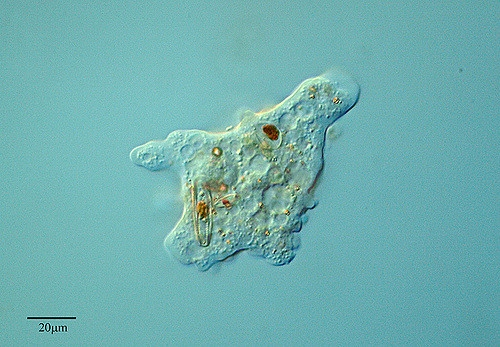
\includegraphics[width=\textwidth]{Eukaryotes1}
	\end{subfigure}
	\begin{subfigure}[b]{0.45\textwidth}
		\caption{ }
		\label{figs:Cellular:predators:symbiotic:hosts2}
		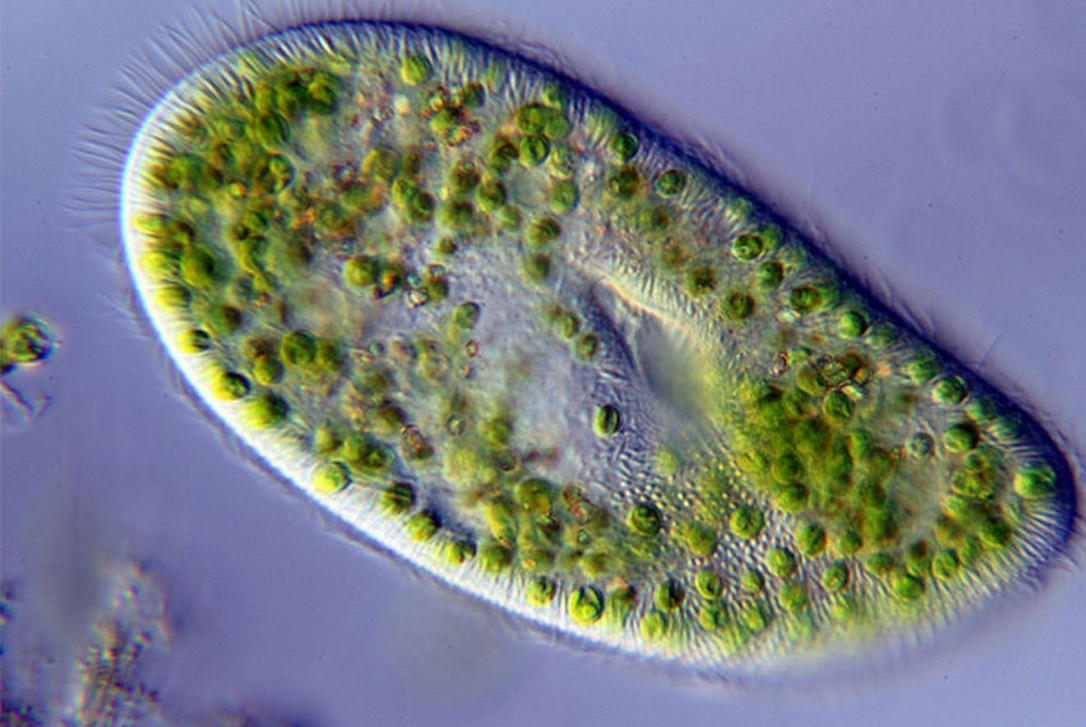
\includegraphics[width=\textwidth]{Eukaryotes2}
	\end{subfigure}
\end{figure}
Why eukaryotes? There are three ideas at present.

\begin{itemize}
	\item Mitochondria improve energetic efficiency, and allow energy use to be regulated more nimbly.\cite{lane2010energetics}.
	
	\item Flexible membranes allow phagocytosis and generation of internal vesicles. So eukaryotes can do things that prokaryotes can't, such as engulfing food prey--Figure \ref{fig:engulf}.
	
	\item Nucleus and endomembrane system allow for finer gene
	regulation--Figure \ref{fig:finer:gene:regulation}\cite{paez2016endocytosis}. Multicellular organization requires different cells to express different parts of the genome. The different layers of regulation may explain why eurkaryotes, and not prokaryotos, have evolved multicellularity.
\end{itemize}

\begin{figure}[H]
	\caption{Flexible membranes allow phagocytosis and generation
		of internal vesicles}
	\label{fig:engulf}
	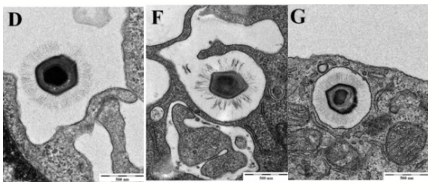
\includegraphics[width=0.9\textwidth]{Engulf}
\end{figure}


\begin{figure}[H]
	\caption{Nucleus and endomembrane system allow for finer gene
		regulation}\label{fig:finer:gene:regulation}
	\begin{subfigure}[b]{0.45\textwidth}
		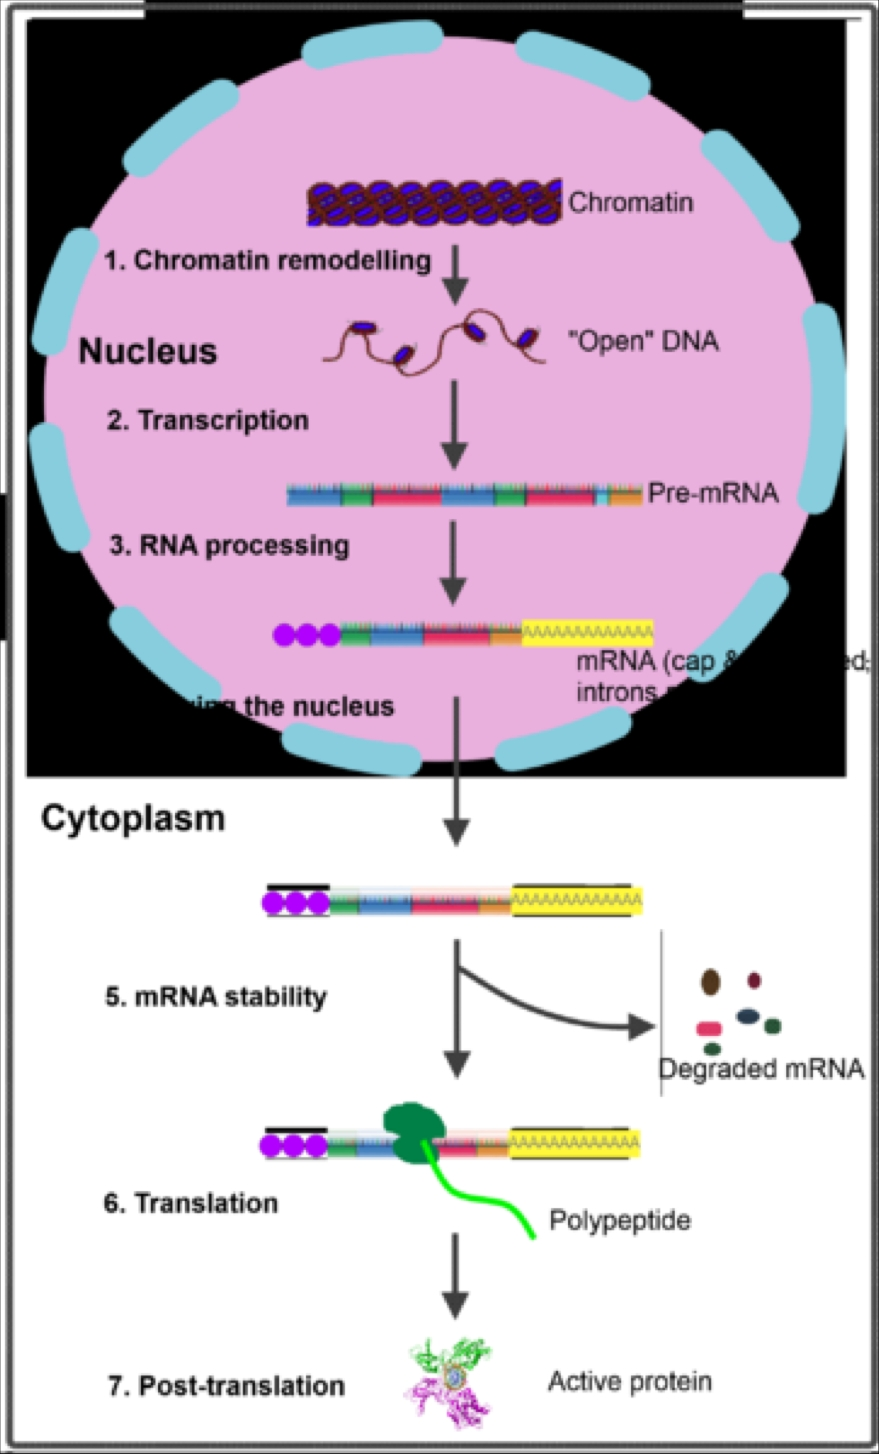
\includegraphics[width=\textwidth]{Regulation1}
	\end{subfigure}
	\begin{subfigure}[b]{0.45\textwidth}
	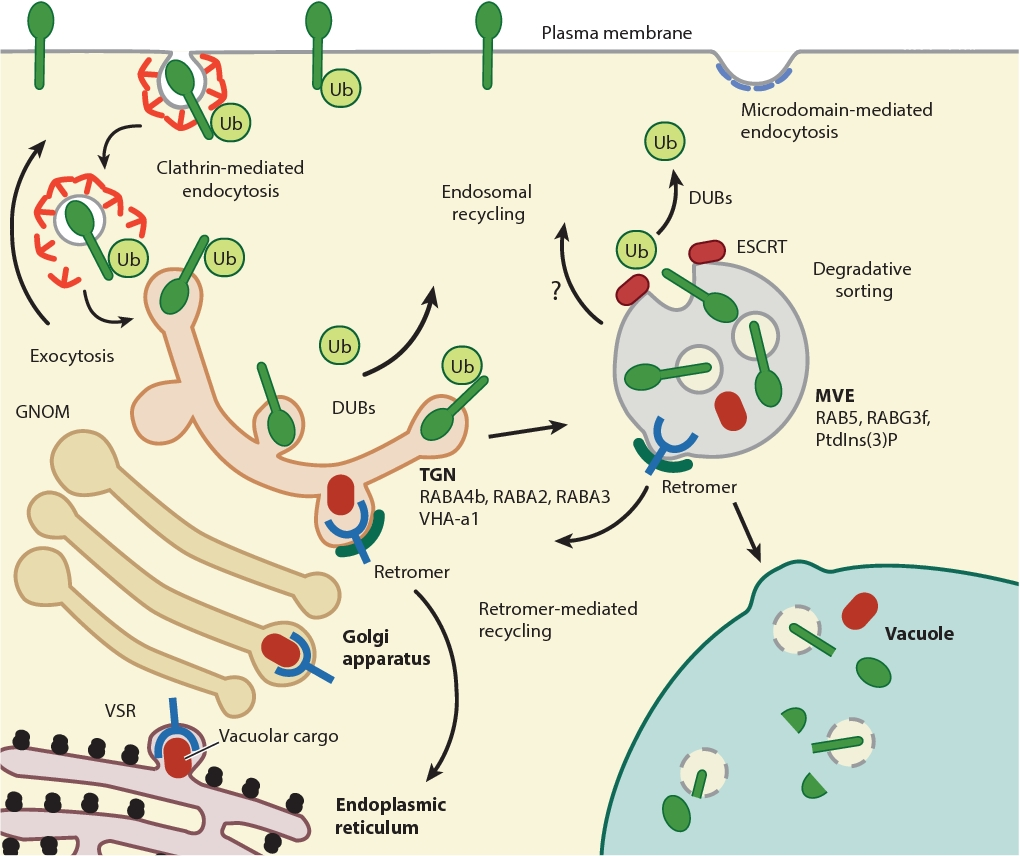
\includegraphics[width=\textwidth]{Regulation2}
	\end{subfigure}
\end{figure}
Easier to study than the
origin of life

\begin{itemize}
	\item We can use phylogenetic methods to infer the features of \gls{gls:LECA}--Figure \ref {fig:LECA}. We can study both ends of the \gls{gls:LECA} branch, since we have procaryotes. Cannot do this with \gls{gls:LUCA}.
	\begin{itemize}
		\item Mitochondria are endosymbiotic bacteria\cite{germot1996presence}
		\item Host was an archaeon\cite{spang2015complex}
		\item Can distinguish genes of archaeal or
		bacterial ancestry\cite{thiergart2012evolutionary}
	\end{itemize}
\end{itemize}

\begin{figure}[H]
	\caption{LECA}\label{fig:LECA}
	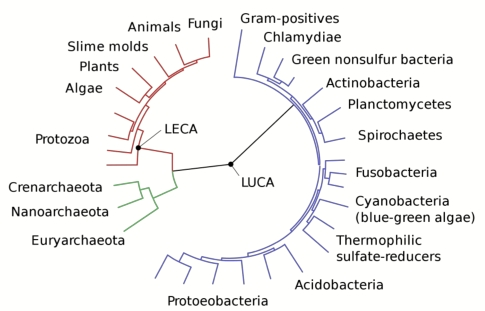
\includegraphics[width=0.9\textwidth]{LECA}
\end{figure}

\begin{figure}[H]
	\caption{Mitochondria are endosymbiotic bacteria}
	\label{fig:Mitochondria:are:endosymbiotic:bacteria}
	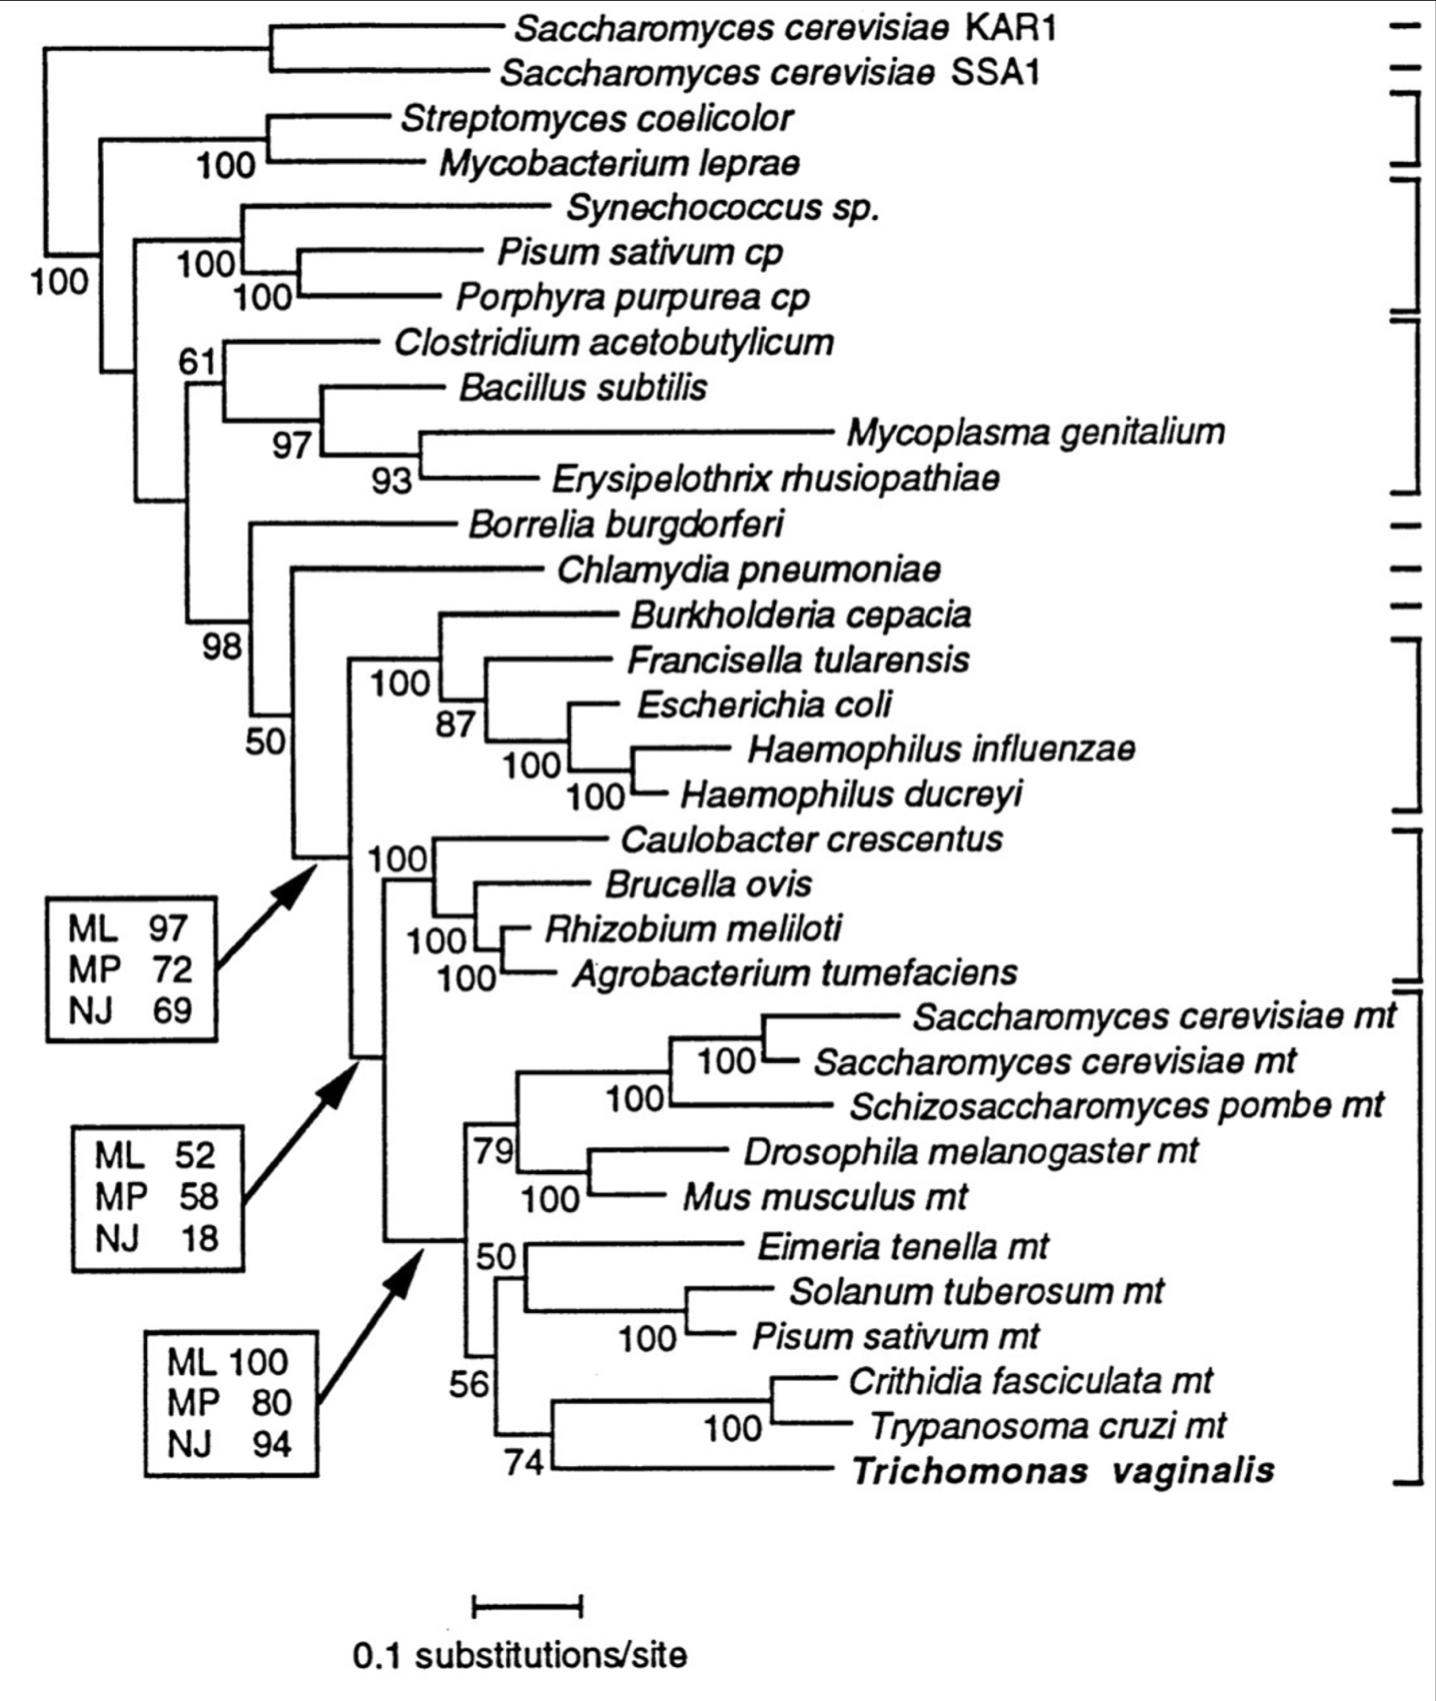
\includegraphics[width=0.9\textwidth]{MitochondriaEndosymbiotic}
\end{figure}

\begin{figure}
	\caption{Host was an archaeon}
	\label{fig:host:archaeon}
	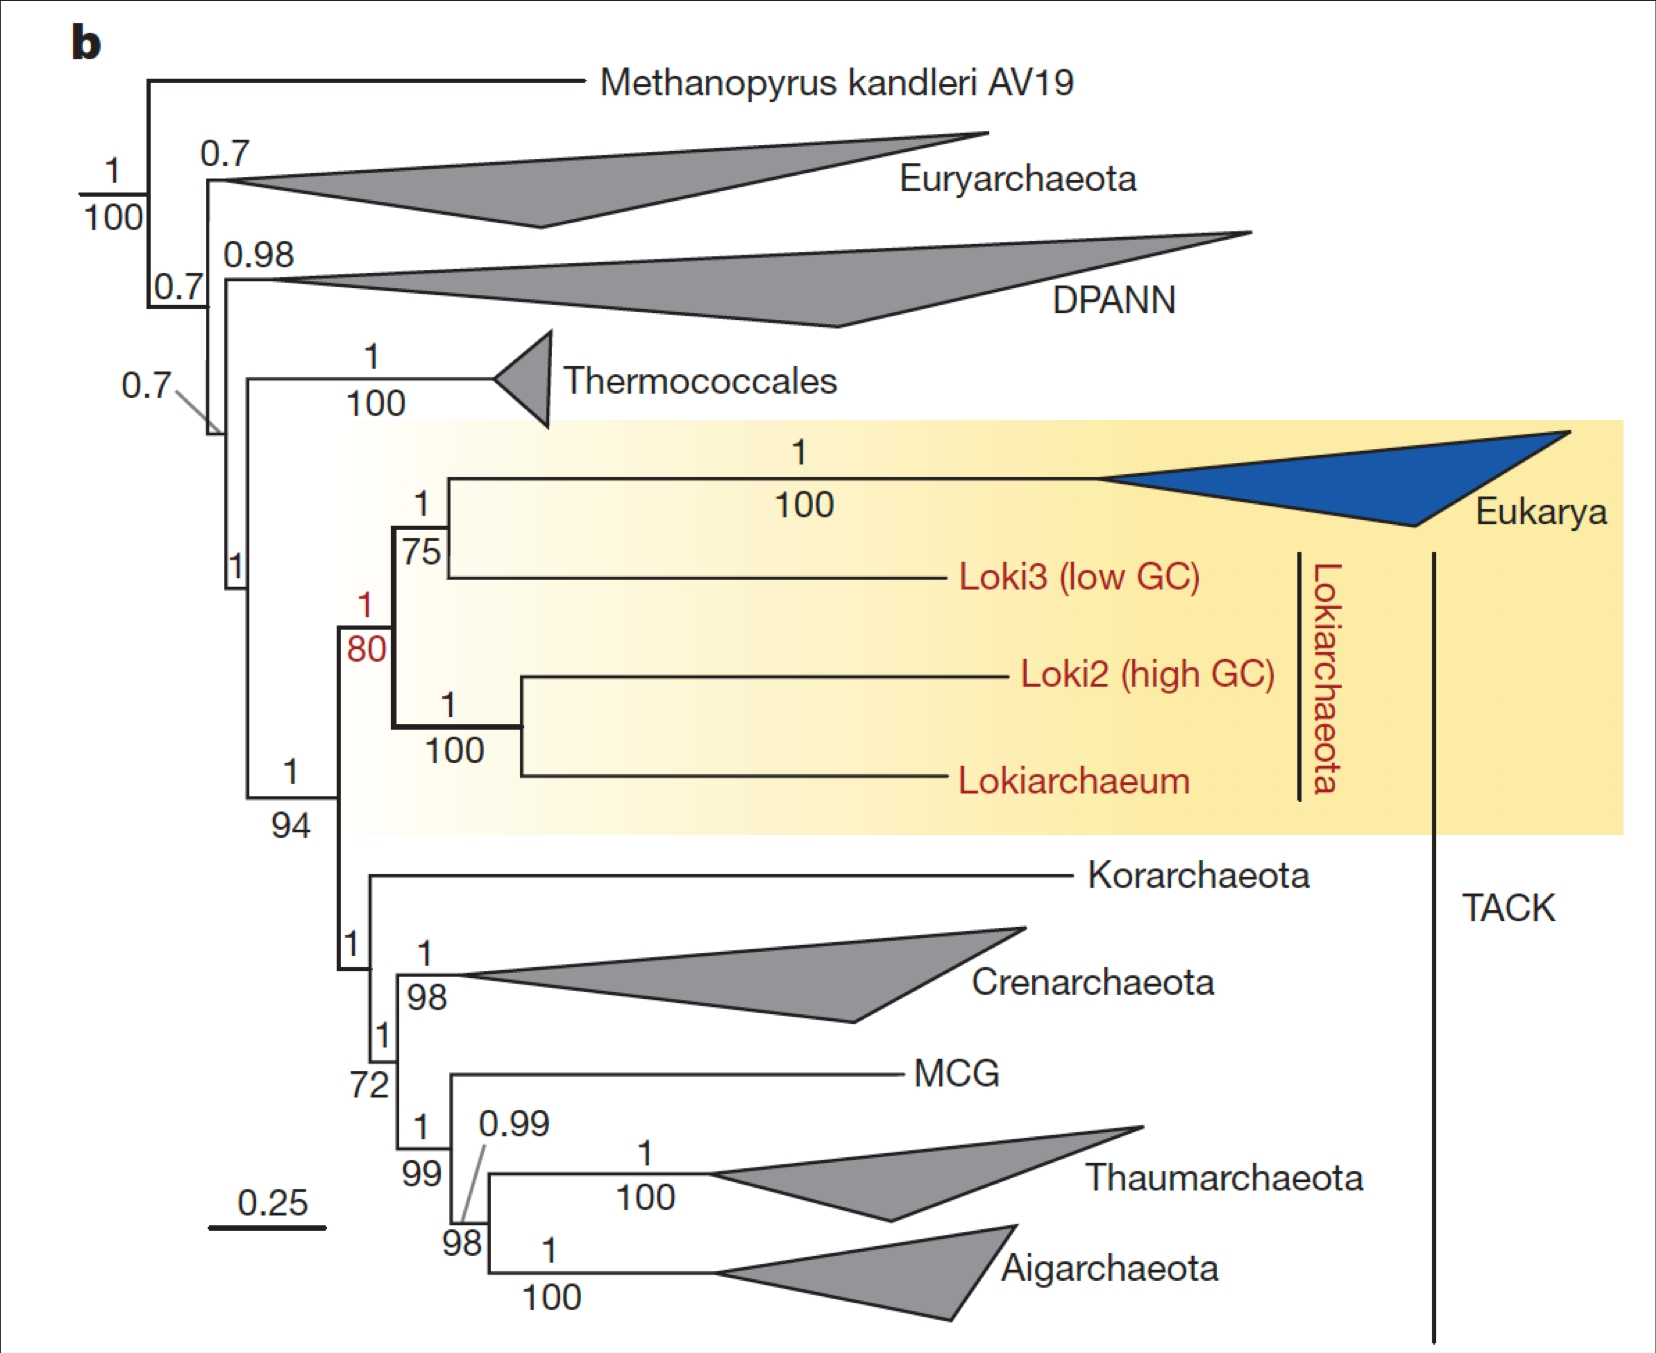
\includegraphics[width=0.9\textwidth]{HostArchaeon}
\end{figure}

\begin{figure}
	\caption{Can distinguish genes of archaeal or bacterial ancestry}
	\label{fig:distinguish:genes:archaeal:bacterial}
	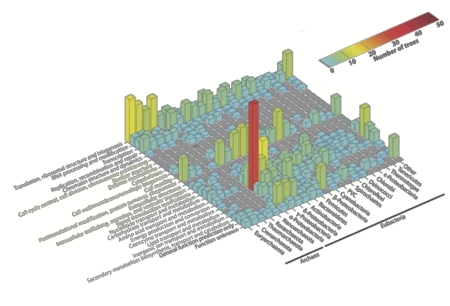
\includegraphics[width=0.9\textwidth]{thiergart2012}
\end{figure}

Mysteries remain
\begin{itemize}
	\item How did a bacterium get into an archaeon? There are two extremes in a range of theories.
	\begin{itemize}
		\item In the Outside-in Model, and archaean developed a membrane, Figure \ref{fig:outside:in1}, which became invaginated. It enveloped mitochondria in a mutualistic association--Figure \ref{fig:outside:in2}. Later it developed membranes to protect DNA from the activity (free oxygen) of the mitochondria--Figure \ref{fig:outside:in3}--until the nucleus was fully enclosed--Figure \ref{fig:outside:in4}.
		\item In the Inside-out Model--Figure \ref{fig:inside:out}--the cell becomes associated with arachaea, which are gradually walled in \cite{baum2014inside}.
	\end{itemize}
	\item How was a nucleus formed?
\end{itemize}

\begin{figure}[H]
	\caption{Outside-in Model}\label{fig:outside:in}
	\begin{subfigure}[b]{0.45\textwidth}
		\caption{ }\label{fig:outside:in1}
		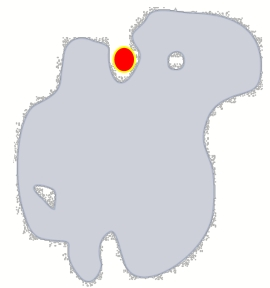
\includegraphics[width=\textwidth]{OutsideIn1}
	\end{subfigure}
	\begin{subfigure}[b]{0.45\textwidth}
		\caption{ }\label{fig:outside:in2}
		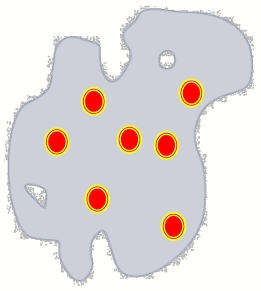
\includegraphics[width=\textwidth]{OutsideIn2}
	\end{subfigure}
	\begin{subfigure}[b]{0.45\textwidth}
		\caption{ }\label{fig:outside:in3}
		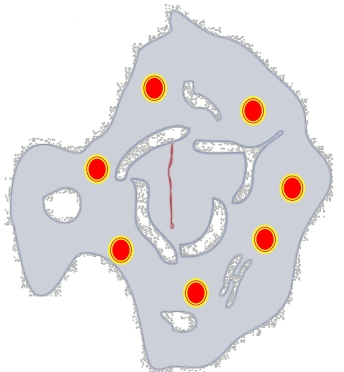
\includegraphics[width=\textwidth]{OutsideIn3}
	\end{subfigure}
	\begin{subfigure}[b]{0.45\textwidth}
		\caption{ }\label{fig:outside:in4}
		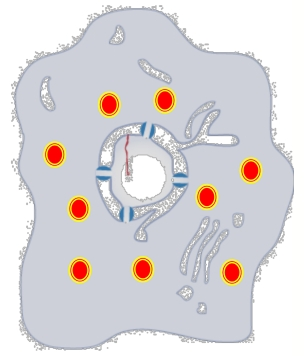
\includegraphics[width=\textwidth]{OutsideIn4}
	\end{subfigure}
\end{figure}

\begin{figure}[H]
	\caption{Inside-Out Model}\label{fig:inside:out}
	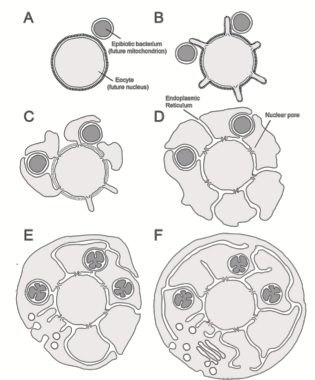
\includegraphics[width=0.9\textwidth]{InsideOut}
\end{figure}

But still easier to solve than the origin of life!
\begin{itemize}
	\item New genomic data keep emerging
	\item There is a possibility of finding intermediates
\end{itemize}

\cite{javaux2003recognizing},  

\section{\Gls{gls:phylogenetics}}


\subsection{Using Phylogenetics to Travel in Time}
Lecturer: Bet{\"u}l Ka{\c c}ar

Key Points
\begin{itemize}
	\item A phylogenetic tree demonstrates evolutionary
	relationships among genes, proteins or organisms.
	\item In a phylogenetic tree, two species are closely
	related if they have a more recent shared ancestor.
\end{itemize}

\cite{hillis1996molecular}, \cite{zuckerkandl1965molecules}, \cite{williams2006assessing}, \cite{woese2002evolution}

\subsection{A Deeper Dive into Phylogenetics}

\cite{huelsenbeck2001mrbayes}, \cite{huelsenbeck1997phylogeny}, \cite{hug2016new}, \cite{philippe2005heterotachy}, \cite{quast2012silva}, \cite{sanderson2003r8s}, \cite{smit2007evolutionary}

\section{Macroscopic Theories in Biology}

\cite{white2005allometric}, \cite{west1997general}, \cite{kempes2011predicting}, \cite{kempes2016evolutionary}
\section{Selection}

\cite{darwin1859origin}

\section{Artificial Life Theory}

\cite{neumann1966theory}, \cite{neumann1958computer}, \cite{janzing2010there}, \cite{schaeffer2014physicallyuniversal}

% end of text 

% glossary
\printglossaries

% bibliography go here
 
\bibliographystyle{unsrt}
\addcontentsline{toc}{section}{Bibliography}
\bibliography{origins}

\end{document}
